\documentclass{mcmthesis}
\mcmsetup{CTeX = false,
        tcn = 2311153, problem = C,
        sheet = true,
        titleinsheet = true,
        keywordsinsheet = true,
        titlepage=false,
        abstract=true}
\usepackage[T1]{fontenc}
\usepackage{palatino}
\usepackage{lipsum}
\usepackage{overcite}
\usepackage{subfig}
\usepackage{amsmath}
\usepackage{multirow}
\usepackage{graphicx}
\usepackage{longtable}
\usepackage{amssymb}
\usepackage{setspace}
\usepackage{wrapfig} 
\usepackage{appendix}
\usepackage{xcolor}
\usepackage{tikz}
\usepackage{pgfplots}
\usepackage{tabularray}
\usepackage{float}
\usepackage{indentfirst}
\usepackage{diagbox}
\usepackage{titlesec}
\usepackage{titletoc}
%\geometry{a4paper,left=2cm,right=2cm,top=2cm,bottom=2cm}
\graphicspath{{figures/}}
\titlecontents{section}
[0.6cm]
{\bf}
{\contentslabel{1.2em}}
{}
{\titlerule*[0.5pc]{$\cdot$}\contentspage\hspace*{0cm}}

\titlecontents{subsection}
[1.3cm]
{}
{\contentslabel{2em}}
{}
{\titlerule*[0.5pc]{$\cdot$}\contentspage\hspace*{0cm}}
\newcommand{\itemEq}[1]{
	\begingroup
	\setlength{\abovedisplayskip}{0pt}
	\setlength{\belowdisplayskip}{0pt}
	\parbox[c]{\linewidth}{\begin{flalign}#1&&\end{flalign}}
	\endgroup}
\setlength{\parindent}{2em}
\title{\textbf{Interstellar: A Global Equity Evaluation Model and Its Application on Asteroid Mining} }
\author{A \and B \and C}
\date{\today}

\makeatletter
\newcommand{\upcite}[1]{\textsuperscript{\textsuperscript{\cite{#1}}}}
\makeatother

% Created by Zu Wang 2022.12.20, I have changed it into the 2023 template, feel free to use it!

\begin{document}
\begin{abstract}
	\small
    \hfill \emph{``We use math to describe the vastness of space, the shape of time, the weight and worth of a human soul.''}

    \hfill ---\emph{Foundation}

The development of space resources is on the schedule of many countries. Resources acquired from various celestial bodies can have a profound impact in all walks of life. However, due to the disparity between countries in technology and economy, many countries may lose the opportunity of getting those resources. A global equity evaluation model should be built and applied on asteroid mining in order to promote global equity.

To begin with, we provide our definition of global equity. \textbf{Global Equity } stands for: All countries have the ability to provide its people with sufficient \textbf{Protection}, \textbf{Education} and \textbf{Economic Resources} during their development.

Then, we establish our \textbf{Global Equity Evaluation Model} based on \textbf{Optimized Cline Function}. The function covered the three aspects we described in our definition. It aims to calculate \textbf{Country Ability Index} which reflects each country's ability to provide these resources to its people. We selected 11 inferior indicators for the three aspects and uses \textbf{Entropy Weight Method} to determine the weight of each indicator. Among all the indicators, the weight of \textbf{Energy} is rising sharply over time which emphasizes the importance of space resources. After determining the weight of each indicator, we apply the \textbf{TOPSIS Method} to grade each section and use Optimized Cline Function to calculate the country ability index. We get the score of 74 countries with USA scoring 0.247 topping the list while Philippines scoring 0.033 ranks at the bottom. 

Next, we use the country ability index to determine a \textbf{Standard Line}. Countries beneath the standard line are considered not capable of providing enough protection, education and economic resources to its people. We create the \textbf{CAID Function} to calculate the \textbf{Global Equity Index}. The idea behind this function is to calculate the sum of the distances between the below-line countries and the standard line. We find out that the global equity index is growing slowly from 0.48 to 0.59 in the last 20 years.

After that, we propose the \textbf{Asteroid Mining Model} to describe and justify our proposed future of asteroid mining. In our model, the \textbf{Asteroid Mining Union} will do the mining , all the countries can fund. We combine the country ability index in the global equity distribution to determine the \textbf{Benefit Distribution Method} and quantify its \textbf{Impact} on global equity.

Finally, we analyze the possible \textbf{Changes} in our proposed future by using \textbf{The Game Matrix}. We also propose \textbf{Policies} targeted for \textbf{Different Time Period}. Sensitivity analysis, the strengths and weaknesses of the models are discussed at the end of the paper.

	\begin{keywords}
		\footnotesize
Optimized Cline Function, Country Ability Index, Global Equity Index, CAID Function, Asteroid Mining Model, Entropy Weight Method
	\end{keywords}
\end{abstract}
\maketitle

\begin{spacing}{0.05}
	\tableofcontents
\end{spacing}
\clearpage
\normalsize

\section{Introduction}
\subsection{Background}
A web-based word game called \textbf{Wordle} rapidly got  popularity at the beginning of 2022, attracting the players by its neatness, high playability. Although the history of word-guessing game can be traced back to 1955, the age of the Internet gives new birth to it, making Wordle play an important role in both personal recreation and social networks\cite{article1}. With one puzzle a day, players only need to take three minutes every day to enjoy the game and have fun competing with their friends for fewer turns to work it out. Hard Mode is also provided for more professional players who wants to challenge themselves. 
\par Due to various attributes of words, data has shown that people tend to have a different distribution for tries with regard to the solution word. Since the popularity of Wordle also changes with time, the total number scores and scores on Hard Mode vary accordingly.

\subsection{Problem Restatement}
\begin{itemize}
\item[$\bullet$] Design a mathematical model to explain the variation of the number of reported results, and make a prediction on a certain day in the future by applying the model. Find relationship between certain attributes of solution words and the percentage of scores reported that are played in Hard Mode.
\item[$\bullet$] Develop a model to predict the distribution of the reported results for a future date. Make uncertainty analysis of the model and the predictions, and apply it to a real case (for the word EERIE on March 1, 2023). Then, evaluate the degree of confidence of the model we develop.
\item [$\bullet$] Develop a model to tell the solution words apart by difficulty. Then, based on the model, identify the attributes of a given word (e.g. EERIE) and quantify its difficulty of guessing it to match it with the classification we make. Finally, make accuracy analysis of the model.   
\item [$\bullet$] Discuss about other interesting features of the data provided.
\end{itemize}
\subsection{Our Contribution and work}

\section{Assumptions and Notations}
\subsection{Assumptions}
$\bullet$ Assume that the results reported from each player were independent to each other, and the trial times distributions for each player were roughly the same.

$\bullet$ Assume that the trial times larger than 7 can be treated as 7 times for simplification of our model because whether exactly 7 times or more won't affect our model much. 
\subsection{Notations}

\begin{longtable}{cc}
	\caption{Notations} \\
	\toprule[2pt]
	Symbols        & Description   \\
	\midrule
	$N_{total}(t)$ & The number of results at the $t^{th}$ day\\
	$N_{hard}(t)$& The number of results in hard mode at the $t^{th}$ day\\
	$N_{Uptrend}(t)$&The number of results for uptrend part at the $t^{th}$ day\\
	$N_{Downtrend}(t)$&The number of results for downtrend part at the $t^{th}$ day\\
	$N_{predict}$&The prediction number of results on March 1, 2023\\
	$n$&The total number of words in the data set.\\
	$word_{i}$& The $i^{th}$ word in the data set.\\
	$X_{vow}$ & The number of Vowel in a word\\
	$X_{rep}$       & The multiplicity of repeated letters\\
	$X_{freq}$    & The  frequency of the word in daily use\\
	$X_{entropy}$      &  Entropy of the word\\
	$X_{ratio}$      &  Ratio of Hard-Mode players among all players on that day \\
	$R_{word-ratio}$& Correlation between word attributes and Hard-Mode Ratio\\
 $\mu_{i}$ & The mean value of trial time results of the $i^{th}$ word\\
 $\sigma_{i}$ &The variance of trial time results of the $i^{th}$ word\\
 $t_{i,j}$&The percentage of results of j trial times cases of the $i^{th}$ word\\
 $w_{i}$& The weight for $t_{i}$ when assessing the difficulty level\\
 $s_{i}$& The weighted distribution score for the $i^{th}$ word.\\
  $x_{i}$& The vector of the $i^{th}$ word projected to $\mathbb{R}^{2}$ for classification \\
  $c_{i}$& The group center for the $i^{th}$ difficulty level.\\
  $U_{i}$& The $i^{th}$ difficulty set.\\
  $u_{i\,j}$& The membership degree for the $i_{th}$ word to the $j^{th}$ difficulty set. \\
  $m$&Fuzzy exponent that determines the fuzziness of difficulty boundaries.\\
  $level_{i}$&The difficulty level the $i^{th}$ word belongs to.\\
  $Accuracy_{cls}$&The accuracy for difficulty classification\\
	\bottomrule[2pt]

\end{longtable}
\par 

\section{Task 1: Time Series and Correlation Analysis}
\subsection{Results Number Variation Model}
\subsubsection{Exponential Curve Fitting Model}
Observing the results number time series, it's conspicuous that the number experiences a variation that it ascended to its peak and then descended with declining acceleration and persistent fluctuation, which indicated a declining popularity of Wordle Game.

To explain the variation, the results number variation can be divided to two parts:

\begin{itemize}
\item [$\bullet$]Part 1: Gradual and continuous increase of new-coming players.
\item [$\bullet$]Part 2: Players leaving the game or playing the game at lower frequencies.

\end{itemize}

Therefore the results number can be summarized in one formula: 
\begin{align}
    N_{Total}(t)=N_{Uptrend}(t)+N_{Downtrend}(t)
\end{align}
\par For Part 1, the rate of the increase of new-coming players is assumed to be linear proportional to the number of new-coming players:
\begin{align}
    \frac{\mathrm{d}}{\mathrm{d}t}N_{Uptrend}(t)=k_{Up}N_{Uptrend}(t)
\end{align}

Then, $N_{Uptrend}(t)=C_{1}\,e^{k_{1}\,t}$, where $C_{1}$ and $k_{1}$ are constant coefficients.

    


For Part 2, the declining trend of popularity resembled the physical cooling process. Studies have shown that this cooling process could be applied in economics or other fields to describe long term dynamics\cite{article2}. \textbf{Newton's law of cooling} has it that the speed of cooling is proportional to the temperature variation, 
\begin{align}
    \frac{\mathrm{d}}{\mathrm{d}t}N_{Downtrend}(t)=-k_{Down}(N_{Downtrend}(t)-N_{Downtrend}(t_0))
\end{align}

Then $N_{Downtrend}(t)=C_{2}\,e^{k_{2}\,t}$, where $C_{2}$ and $k_{2}$ are constant coefficients.

Therefore, the $N_{Total}(t)$ has the form:
\begin{align}
    N_{Total}(t)=C_{1}\,e^{k_{1}\,t}+C_{2}\,e^{k_{2}\,t}
\end{align}

Fit the curve and then came the results:
\begin{align}
    N_{Total}(t)=544900\,e^{-0.01755\,t}+18760\,e^{0.0007413\,t}
\end{align}

The R-square is 0.9873, which is quite close to 1, suggesting the excellent fitting effect.
\begin{figure}[h]
    \centering
    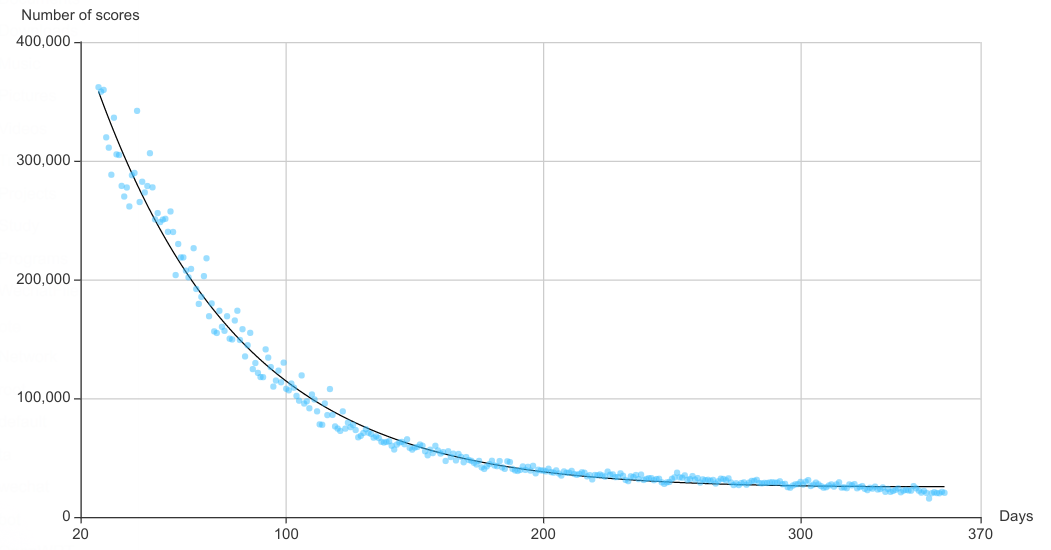
\includegraphics[scale=0.55]{expfit.png}
    \caption{Fitting Curve for Results Number}
    \label{fitting curve}
\end{figure}

\subsubsection{LSTM Prediction Model}
\par The \textbf{exponential fitting curve model} can explain the variation of number of players in a large scale, but the \textbf{smooth curve} it gives leaves out the \textbf{fluctuation information} of data. Therefore, we resorted to LSTM Prediction Model for more practical predictions, since the machine learning algorithm can study the details of fluctuations and flows.

\begin{figure}[h]
    \centering
    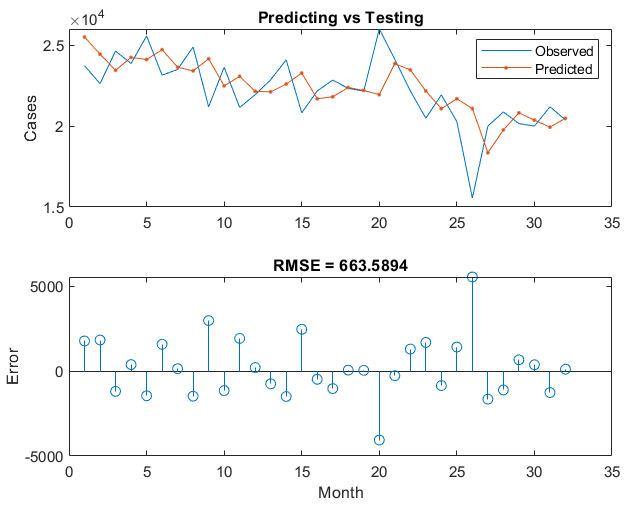
\includegraphics[scale=0.78]{LSTM_total.png}
    \caption{LSTM Prediction: Predicting Results and Testing data}
    \label{LSTM Graph}
\end{figure}

The data of results number was split to $90\%$ training set and $10\%$ testing set. As can be seen from Figure \ref{LSTM Graph}, the predicting results were quite consistent with the testing data, and \textbf{RMSE=663.5894}.

Further predicted the results numbers for next 60 days, and the predicting results number for March 1, 2023 was \textbf{15315}.

Then we applied \textbf{Hypothesis Testing} for calculating the prediction interval at the $\alpha=0.1$ significance level.

\begin{figure}[h]
    \centering
    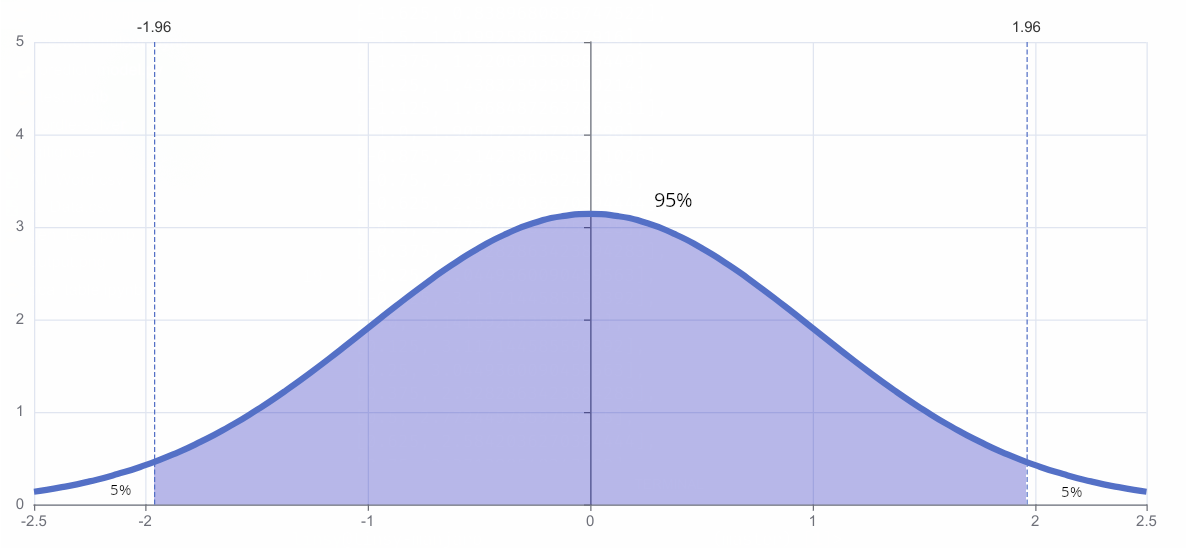
\includegraphics[scale=0.5]{dist.png}
    \caption{Normal Distribution with Labeled Probability}
    \label{norm dist}
\end{figure}

To accept the hypothesis that $N_{Predict}$ is a possible result, $N_{Predict}$ should satisfy the inequality that
\begin{align}
    \phi(|\frac{N_{predict}-15315}{RMSE}|)\leq 97.5\%
\end{align}
where $\phi(x)$ is the PDF for normal distribution, and then
\begin{align}
    |\frac{N_{predict}-15315}{RMSE}|\leq 1.96
\end{align}

Therefore, the prediction interval for $N_{predict}$ is \textbf{[14014,16616]}.

\subsection{Correlation Analysis}
\subsubsection{Word Attributes Model}
In order to explore how \textbf{word attributes} affect the percentage of scores 
played in Hard Mode, we first introduce 4 indications that feature the word. Different words have their own attributes to make them unique. Throughout the paper, we mainly focus on 4 attributes of words that may \textbf{influence players' trial times for guessing}.

\begin{itemize}

    \item [$\bullet$] Vowel Number ($X_{vow}$) : The number of vowels in a word will influence its difficulty to be guessed. Since all words have vowels and there are only five of them among the alphabet, players are more likely to guess words based on them.
    
    \begin{figure}[h]
    \centering
    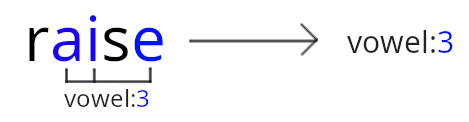
\includegraphics[scale=1.4]{raise.png}
    \caption{Illustration for Vowel Number ($X_{vow}$) }
    \label{norm dist}
    \end{figure}

    \item [$\bullet$] Repetition Number ($X_{rep}$) : Repeated letters appeared in a single word will impact the amount of information it gives out. $X_{rep}$ was calculated by subtracting 1 from highest repetition times for letters in the word.
   
    \begin{figure}[h]
    \centering
    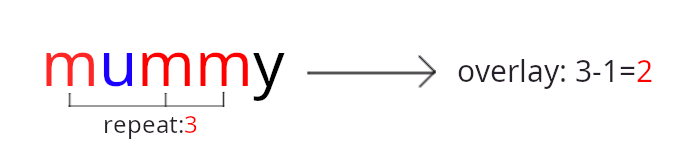
\includegraphics[scale=1.3]{mummy.png}
    \caption{Illustration for Repetition Number ($X_{rep}$) }
    \label{norm dist}
    \end{figure}
    
    \item [$\bullet$] Word Frequency ($X_{freq}$) : The frequency of word used in daily life may directly influence the number of attempts to some extent.
    %%%%%%%%%%%%%%% TODO 词频还需要说什么呀 引用网址
    
    \item [$\bullet$] Information Entropy ($X_{entropy}$) : For this attribute, we learn from the definition of entropy to quantify the information that guessing a certain word can provide. According to Sanderson's algorithm\cite{article3}, the entropy of guessing a word can be represented as the formula:
    %%%%%%%%%%%%%%% TODO 这里需要写成伪代码吗
    
    $$ E[I]=\sum_{x}p(x)\cdot \log_2(\frac{1}{p(x)}) $$
    Where p(x) refers to the probability of each outcome of guessing. For example, if we guess "crane" and the outcome is green on "c" and yellow on "a", the p(x) in this case refers to all possible words that satisfy this constraint divided by the number of all five-letter words in database.
\end{itemize}
\subsubsection{Word Attributes $\&$ Hard-Mode Ratio $X_{ratio}$ Correlation Analysis}
    \par In addition to word attributes, we also need to name a factor to represent the percentage of hard mode scores among all the results. 
    \begin{itemize}
        \item [$\bullet$]
    Hard-Mode Ratio ($X_{ratio}$) : We calculate the value of hard-mode results divided by all the results in a day. Our mission is to use models to find how this ration is related to the word attributes mentioned above.
\end{itemize}

The variables $X_{vow}$,$X_{rep}$,$X_{freq}$,$X_{entropy}$ and $X_{ratio}$ were first normalized to eliminate the influence of units by the z-score formula:
\begin{equation*}
    \Tilde{x}=\frac{x-\mu_{x}}{\sigma_{x}}
\end{equation*}

\par Then we calculated covariance and correlation coefficient to evaluate the overall dependency of every two variables by formulas:

\begin{center}
    Covariance: $\mathrm{Cov}(x,y)=E[(X-E[X])\times (Y-E[Y])]$
\end{center}

\begin{center}
    Correlation Coefficient: $r(x,y)=\dfrac{\mathrm{Cov}(x,y)}{\sigma_x\,\sigma_y}$
\end{center}
\par Then the correlation matrix $R_{word-ratio}$ was generated and shown below.
\par Based on the results shown in the matrix, we find that each covariance of $X_{Ratio}$ with respect to the four word attributes respectively is around 0.1, which indicates that the Hard-Mode ratio are not necessarily affected by word attributes. 

It may be naturally explained by the fact that players won't be influenced by words in-game when selecting game modes before-game.

\subsubsection{Results Distribution Model}
To simplify the distribution of trial times varying between words, based on the abundance of data source and the assumption that the trial times between players are independent and followed a roughly same distribution pattern, we applied \textbf{Central Limit Theorem} and assumed the distribution of trial times to be a \textbf{Gaussian Distribution}.

Therefore, only two variables: \textbf{Mean ($\mu$) and Variance ($\sigma$)} to describe the distribution.

It is worthwhile noticing that the larger Mean ($\mu$) will imply a \textbf{greater difficulty} to guess the word since more trial times are needed.

\subsubsection{Word Attributes and Distribution Correlation Analysis}

\par A covariance matrix was applied again to illustrate the correlation between word attributes and the results distribution.

\par Two conclusions could be reached by the covariance matrix:

(1) The Mean value ($\mu$) is positively correlated to $X_{rep}$, which means that the larger $X_{rep}$ is for a word, the harder it is for players to guess.

\textbf{Possible Explanation:} This coincides with the fact that the more repeated letters a word have, the less probability a player can guess a right letter.

(2) The Mean value ($\mu$) is negatively correlated to $X_{entropy}$, which means that the larger $X_{entropy}$ is for a word, the easier it is for players to guess.

\textbf{Possible Explanation:} The information entropy ($X_{entropy}$) can describe the probability for the word to deduce to other words based on our definition. Correspondingly, it also implies \textbf{how much probability other words can deduce this word}. Therefore, greater information entropy can make the word easier to be guessed,





\section{Task 2: Results Distribution Prediction Model}
\subsection{Principle Component Analysis (PCA) for Word Attributes}
%%%%%% TODO Graph
Observing the correlation matrix, much \textbf{correlation} can be noticed between word attributes. For example, the appearance of overlapped letters and numbers of vowels affect may each other, and may also have an influence on the entropy. 

Based on these discoveries, we came up with the \textbf{Principle Component Analysis (PCA)} for two reasons: 
\begin{itemize}
   \item\textbf{Reason 1: } Convert these highly correlated variables into independent variables.
    \item\textbf{Reason 2: } Project the variables onto lower dimensions to simplify the model and make the problem more solvable. 
\end{itemize}

\begin{table}[htbp]
\begin{tabular}{c c c}
\toprule[2pt]
Eigenvalue & Principle Component&  Accumulated Contribution\\ 
 \hline
 $1.63$ & $0.25X_{vow} - 0.64X_{rep}+ 0.13X_{freq} + 0.71X_{entropy}$  & $40.76\%$ \\
%  \hline
 $1.06$ & $0.80X_{vow} + 0.41X_{rep}+ 0.44X_{freq} + 0.02X_{entropy}$  & $67.33\%$  \\
%  \hline 
 $0.97$ & $-0.44X_{vow} - 0.10X_{rep}+ 0.89X_{freq} - 0.10X_{entropy}$  & $91.63\%$ \\
\bottomrule[2pt]
\end{tabular}
\caption{PCA for word attributes}
\end{table}
%%%%% TODO: visualize

\subsection{Backpropagation (BP) Neural Network}

The distribution of game result is a vector in seven dimension (from one guess to more than 6 guesses), and the game input is the word and the ratio of hard-mode player. The relationship between them is difficult to find. BP neural networks are capable of modeling nonlinear relationships between the input data and the output. This is important in the Wordle result distribution prediction model because the feedback given by the game is based on complex rules and is not directly related to the solution word. BP neural networks can find those complex characteristics by backpropagation.

\subsubsection{Data Pre-process}

After using the PCA for all words, the four word attributes can be converted to \textbf{three principle components} $Y_1, Y_2, Y_3$. The input layer of the BP neural network has four neurons: $Y_1, Y_2, Y_3$, and the hard-mode ratio $X_{ratio}$.

By fitting the discrete distribution of game result with the continuous normal distribution,we can prepare the samples of the output layer that has two neurons: $\mu$ and $\sigma$, which can be used to generate the equivalent normal distribution result.

\subsubsection{Network Structure}

To better fit the sample data set, we tried different study rate, number of layers and number of nodes in hidden layers. We also take the problem of over-fitting into account and finally determined to use the 4-6-6-2 neural network. We choose to use the $\mathrm{ReLU}$ activation function : $\mathrm{ReLU}(x) = \begin{cases}
    x,  x> 0\\
    0, x\leq 0
\end{cases}$ between adjacent linear layers which can improve the nonlinear fitting ability of our model.

We choose to use the \emph{Mean Squared Error} (\textbf{MSE}) function as the loss function of our network:
\begin{align}
    \mathrm{MSE} = \frac{1}{N}\sum_{i=1}^N(y_i - \hat{y_i})^2
\end{align}

The backpropagation process will use this function to compute the gradient of the error and update the weights and biases of the network by using a gradient descent optimization algorithm.

\begin{figure}[H]
    \centering
    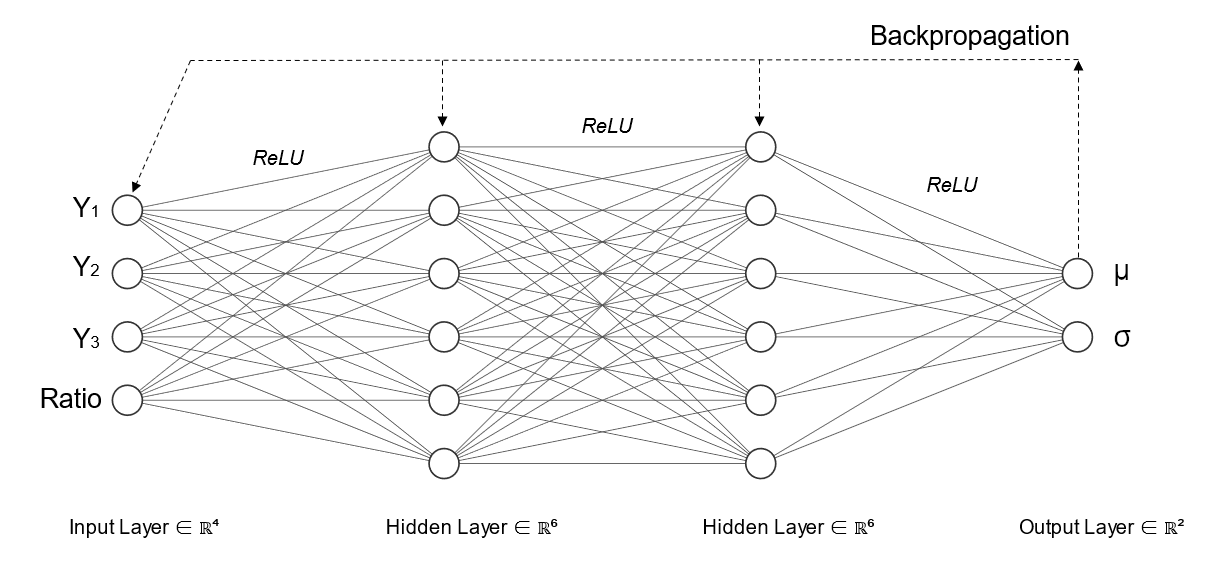
\includegraphics[scale=0.6]{BP.png}
    \caption{The BP Neural Network Structure}
\end{figure}

\subsection{Validation of the Model}

After training this BP neural network for $10^6$ iterations, the total MSE loss has been reduced to about $0.074$.

To validate the model's robustness, we divided the sample data into training set and testing set. The training set conrains 80\% of the data while the testing set contains 20\% of the data. We first train our model on the trainging set then test it on the testing set and compare the MSE loss of two sets. We randomly choose those two sets for 6 times and the result is shown in figure \ref{Train Set}. The difference between the training set and the testing set is about 10\% of the training set MSE loss, which is acceptable.

\begin{figure}[H]
    \centering
    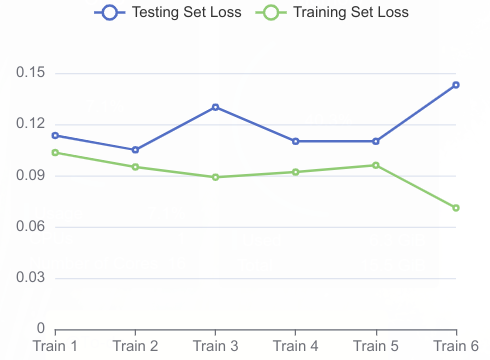
\includegraphics[scale=0.5]{trainingloss.png}
    \caption{MSE Loss of Training and Testing Set}
    \label{Train Set}
\end{figure}

\section{Task 3: Word Difficulty Classification and Prediction}
\subsection{Weighted Distribution Scoring Model}
To better measure the difficulty of the word by the result distribution of trial times, it is meaningful to assign different weights to different trial times and calculate weighted trial times for 2 reasons:
\begin{itemize}
    \item\textbf{Reason 1: } For most words, most people try 3-5 times to guess, so the trial times between 3-5 usually can't provide valuable information for assessing difficulties.
    
    \item\textbf{Reason 2: } Though relatively few people guess the words for just 1~2 times or more than 6 times, those cases are actually most valuable for assessing difficulties.
\end{itemize}

The goal of \textbf{rating information value and assigning weight} for $t_{i} (i=1,2...,7)$ reminded us of applying \textbf{Entropy Weight Method}. Entropy Weight is found to enhance the function of the attribute with the highest diversity of attribute data (DAD) as well as weaken the function of the attributes with a low DAD in decision-making or evaluation.
\par Since we have n words and 7 indicators to be weighted, we generated the data matrix:
\begin{align}
	X=\left[\begin{array}{cccc}
			t_{11}  & t_{12}  & \cdots & t_{17} \\
			t_{21}  & t_{22}  & \cdots & t_{27} \\
			\vdots  & \vdots  & \ddots & \vdots  \\
			t_{n 1} & t_{n 2} & \cdots & t_{n7}
		\end{array}\right]
\end{align}
\par Then we standardized the data we have and got the standardized matrix $Z=(\tilde{t}_{i j})$,
\begin{align}
	\tilde{t}_{i j}:=\frac{t_{i j}}{\sqrt{\sum\limits_{k=1}^{n} t_{k j}^{2}}}
\end{align}
\par Next, we normalized the data and got the probability matrix $P=(p_{i j})$. 
\begin{align}
	p_{i j}:=\frac{\tilde{t}_{i j}}{\sum\limits_{k=1}^{n} \tilde{t}_{k j}}
\end{align}
\par Finally, we calculated the information entropy and the entropy weight of $t_{i}$ $(i=1,2,...,7)$.
\begin{align}
	e_{j}:=-\frac{1}{\ln n} \cdot \sum_{i=1}^{n} p_{i j} \ln p_{i j}    \quad w_{j}=\frac{1-e_{j}}{\sum\limits_{i=1}^{m} (1-e_{j})}, j=1,2,...,7
\end{align}
\par The \textbf{Weighted Distribution Score} for the $j^{th}$ word is then:
\begin{align}
    s_{i}=\sum_{j=1}^{7}w_{j}\,t_{i\,j}
\end{align}

Generally, a larger weighted distribution score means a greater word difficulty.


%%%%%%%% TODO 计算步骤和可视化美化
\subsection{Word Difficulty Classification Model}

\subsubsection{Difficulty Level Setting}
We set \textbf{4} difficulty Levels for Wordle Game, which were respectively \textbf{Easy, Medium, Hard, Hell} with increasing difficulty. Therefore, the mission is to classify the words given in data set into 4 \textbf{difficulty sets}:

\qquad $U_{1}=\{\text{words} | \text{difficulty = Easy}\}$ \quad $U_{2}=\{\text{words}|\text{difficulty = Medium}\}$

\qquad $U_{3}=\{\text{words} | \text{difficulty = Hard}\}$ \quad $U_{4}=\{\text{words}|\text{difficulty = Hell}\}$

\subsubsection{Indicators for Difficulty Classification}
We select two indicators for difficulty classification:

    (1) \textbf{Trial Time Results Mean ($\mu_{i}$)} \qquad (2) \textbf{Weighted Distribution Score ($s_{i}$)}

Generally, larger $\mu_{i}$ and larger $s_{i}$ indicate higher word difficulty, we believe that considering the distribution of both of them can make our difficulty classification more comprehensive. 

\subsubsection{Word Difficulty Embedding Model}
The words are embedded into $\mathbb{R}^{2}$ vectors. For the $i^{th}$ word, the embedded vector is:
\begin{align}
    x_{i}=(\tilde{\mu_{i}},\tilde{s_{i}})
    \label{z-score}
\end{align}
where $\tilde{\mu_{i}}$ and $\tilde{s_{i}}$ are z-score standardized $\mu_{i}$ and $s_{i}$ 
\subsubsection{Apply Fuzzy C-Means Model (FCM) for Classification}
Since the relationship between words were quite fuzzy, the boundary between each different difficulty modes should be blurred. Therefore, we resorted to \textbf{Fuzzy C-Means Model (FCM)} for word difficulty classification.

First, the centers of four difficulty groups were set to be $c_{i}$, $(i=1,2,3,4)$, and the detailed values were calculated later.

Then, \textbf{Euclidean Distance} was applied for describing the distance between the embedding vectors of words:

\begin{align}
    \mathrm{dist}(c_{i},x_{i})=\|c_{i}-x_{i}\|_{2}
\end{align}



After that, To characterize the fuzziness, we introduced the concept \textbf{membership degree} $u_{i\,j}$,to describe the probability for the $i^{th}$ word to belong to the $j^{th}$ difficulty level:
\begin{align}
    u_{i\,j}=P[word_{i}\in U_{j}]
\end{align}
Since every word must belongs to one difficulty set, we consequently had:
\begin{align}
    \sum_{j=1}^{4}u_{i\,j}=1
\end{align}
Then the \textbf{fuzzy partition matrix} was constructed as $U=(u_{i\,j})$.

Then the target is to minimize the objective function:
\begin{align}
    J(U,C)=\sum_{s=1}^{4}\sum_{i=1}^{n}(u_{is})^{m}\times \mathrm{dist}(c_{i},x_{s})^{2}
    \label{objective-function}
\end{align}
where $m=1.2$ is the arbitrarily-set \textbf{fuzzy exponent} that controls how much the clusters overlap with each other, therefore m describes the fuzziness of difficulty boundaries. 

Then we applied \textbf{Iterative Method} with formulas:
\begin{align}
    u_{i\,j}^{'}=\dfrac{1}{\sum\limits_{k=1}^{4}(\frac{\|x_{i}-c_{j}\|}{\|x_{i}-c_{k}\|})^{\frac{2}{m-1}}}, C_{j}^{'}=\dfrac{\sum\limits_{i=1}^{n}u_{i\,j}^{m}\times x_{i}}{\sum\limits_{i=1}^{n}u_{i\,j}^{m}}
\end{align}
and then the satisfying membership degree matrix $U=(u_{i\,j})$ and centers $C_{i}$ (i=1,2,3,4) were ultimately found to let the objective function (\ref{objective-function}) attain its approximated minimum.

Finally, we classified the words to the difficulty sets to which the words had highest membership degree:
\begin{align}
    \mathrm{level}_{i}=\mathop{\arg\max}_{j} u_{i\,j}
\end{align}

\subsubsection{Accuracy Analysis}
The accuracy for classifying $\mathrm{word}_{i}$,$(i=1,2,...,n)$ can be described by its membership degree $u_{i\,\mathrm{level_{i}}}$.

We calculated the overall accuracy by taking the mean value of accuracy for all the wards in the data set:
\begin{align}
    \mathrm{accuracy}_{cls}=\dfrac{\sum\limits_{i=1}^{n}u_{i\,\mathrm{level_{i}}}}{n}
\end{align}

After examination, we got that $\mathrm{accuracy}_{cls}=96.5\%$, which is really satisfying.
\subsection{Difficulty Classification for Eerie}
With the distribution information acquired in Task 2, the Trial Times Mean and Weighted Distribution Score of "Eerie" can be calculated. We standardized $\mu_{Eerie}$ and $s_{Eerie}$ with the z-score coefficients used in equation (\ref{z-score}) and then we got $\tilde{\mu}_{Eerie}$ and $\tilde{s}_{Eerie}$. Therefore, the embedding $\mathbb{R}^{2}$ vector for "Eerie" is:
\begin{align}
    x_{Eerie}=(\tilde{\mu}_{Eerie},\tilde{s}_{Eerie})
\end{align}

We applied the \textbf{Word Difficulty Classification Model} for "Eerie" and the results were visualized in Figure \ref{cluster}:

\begin{figure}[h]
    \centering
    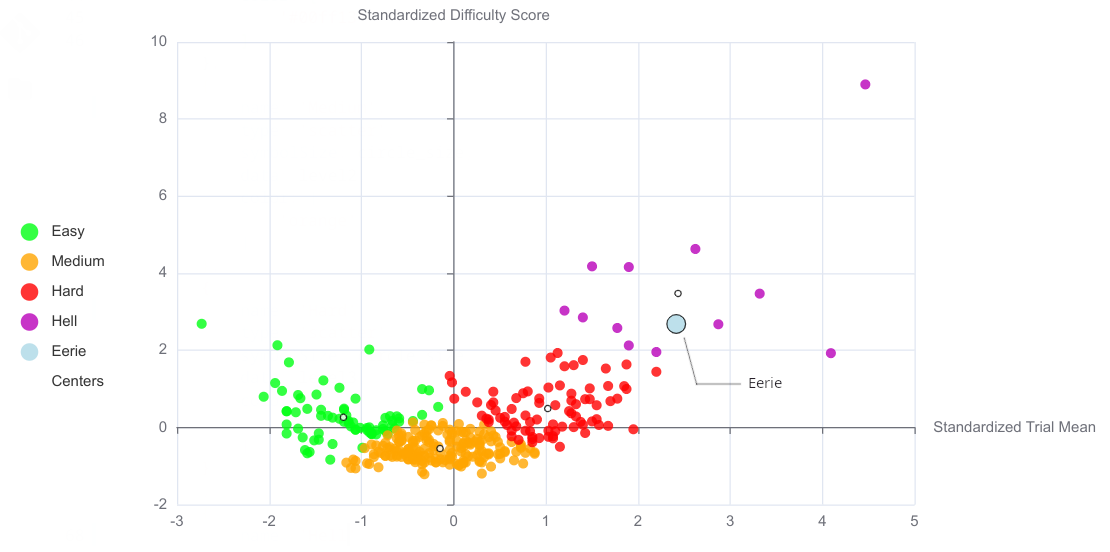
\includegraphics[scale=0.6]{cluster.png}
    \caption{Word Difficulty Classification}
    \label{cluster}
\end{figure}

It can be clearly seen that "Eerie" is classified into the \textbf{Hell Difficulty Category}.

\include{Sensitivity Analysis.tex}
\section{Future Updates for the Model}
\section{Strength and Weakness}
\subsection{Strength}
\subsection{Weakness}
\section{Conclusion}
\addcontentsline{toc}{section}{References}
\begin{thebibliography}{99}
    \bibitem[1]{article1} "Wordle." Wikipedia, Wikimedia Foundation,  en.wikipedia.org/wiki/Wordle. 
    \bibitem[2]{article2} Jadranda D.T.(2018). Applicability of Newton’s law of cooling in monetary economics. Physica A: Statistical Mechanics and its Applications, vol 494, 209-217.
	%\bibitem[1]{article1} The Treaty on Principles Governing the Activities of States in the Exploration and Use of Outer Space, including the Moon and other Celestial Bodies, of 27 January 1967, United Nations RES 2222 (XXI).
	\bibitem[3]{article2} Sanderson. G (2022). Solving Wordle using you keep your information strcak theory. https://www.3bluelbrown.com /lessons /wordle.
	%\bibitem[3]{article3} Desikan, A. Supporting Equity and Environmental Justice.
	\bibitem[4]{article4} Cline, R. S. (1977). World Power Assessment 1977: a Calculus of Strategic Drift.
	\bibitem[5]{article5} Anielski, M. (2002). The Alberta GPI: Economy, GDP, and Trade. Pembina Institute.
	\bibitem[6]{article6} Yitzhaki, S. (1983). On an extension of the Gini inequality index. International economic review, 617-628.
	\bibitem[7]{article7} Mutschler, Max M., and Marius Bales. ``Global Militarisation Index 2019.'' (2019): 15.
	\bibitem[8]{article8} Hart, D. V. (1964). Ethnocentrism and the ``Education Index''. Comparative Education Review, 8(2), 138-140.
	\bibitem[9]{article9} Chen, P. (2021). Effects of the entropy weight on TOPSIS. Expert Systems with Applications, 168, 114186.
	\bibitem[10]{article10} Fialho, D.\& Van Bergeijk, P. A. (2017). The proliferation of developing country classifications. The Journal of Development Studies, 53(1), 99-115.
	\bibitem[11]{article11} Badescu, V. (Ed.). (2013). Asteroids: Prospective energy and material resources. Springer Science \& Business Media.

\end{thebibliography}


\end{document}
